\documentclass[11pt,letterpaper]{article}
\usepackage[utf8]{inputenc}
\usepackage[T1]{fontenc}
\usepackage{lmodern}
\usepackage{geometry}
\usepackage{xcolor}
\usepackage{graphicx}
\usepackage{booktabs}
\usepackage{array}
\usepackage{tabularx}

\geometry{margin=2.2cm,headheight=15pt}
\definecolor{Navy}{HTML}{172033}
\definecolor{Blue}{HTML}{2563EB}
\definecolor{Cyan}{HTML}{06B6D4}
\definecolor{Pale}{HTML}{EFF6FF}
\definecolor{Muted}{HTML}{64748B}
\graphicspath{{../outputs/figures/}}
\pagestyle{plain}
\setlength{\parindent}{0pt}
\setlength{\parskip}{6pt}

\begin{document}

\begin{titlepage}
\pagecolor{Navy}
\color{white}
\vspace*{1.2cm}
{\small UNIVERSIDAD DEL VALLE DE GUATEMALA}\par
\vspace{2.2cm}
{\Huge\bfseries Laboratorio 7}\par
\vspace{0.25cm}
{\fontsize{30}{34}\selectfont Spark MLlib}\par
\vspace{0.7cm}
{\Large Perfiles laborales y predicción salarial con ENEIC}\par
\vspace{1.5cm}
\colorbox{Blue}{\parbox{0.88\textwidth}{\color{white}\centering\large Avance funcional del 75\% · Actividades 1--6 completas}}
\vfill
\begin{tabularx}{\textwidth}{X r}
\textbf{Jorge Gabriel Palacios Sales} & 231385\\[6pt]
\textbf{Pablo Daniel Barillas Moreno} & 22193\\[6pt]
\textbf{Roberto Emiliano Otoniel} & 23968\\
\end{tabularx}
\vspace{1cm}
CC3084 · Data Science · Sección 10 · Grupo 1\\
Segundo semestre 2026
\vspace*{0.7cm}
\end{titlepage}
\nopagecolor
\color{Navy}

\section{Resumen ejecutivo}

Se construyó un flujo reproducible con Python 3.11, Spark 3.5.1 y la API \texttt{pyspark.ml}. El avance procesa las bases oficiales de Personas ENEIC, preserva su procedencia, audita cada exclusión, caracteriza la población analítica, compara segmentaciones KMeans y valida dos familias de regresión mediante una separación temporal. Los resultados son no ponderados y no deben interpretarse como estimaciones oficiales ni relaciones causales.

\subsection{Hallazgos principales}
Después de aplicar los criterios de elegibilidad se conservaron \textbf{53,025} registros de 2025. El salario medio fue \textbf{Q3,421.68} y la mediana \textbf{Q3,000.00}; esta separación evidencia asimetría y la influencia de valores altos.
La asociación lineal absoluta más alta con salario entre los predictores numéricos corresponde a \texttt{antiguedad} ($|r|=0.180$).
KMeans seleccionó \textbf{Perfil laboral (sin salario)} con $K=2$ y silhouette 0.5545.
En validación temporal (2025T4), \textbf{RF\_50\_arboles\_d7} obtuvo el menor RMSE (Q2,074.15).
En la prueba final (2026T1, 13,258 registros), \textbf{RF\_50\_arboles\_d7} obtuvo el mejor desempeño: MAE Q1,141.51, RMSE Q2,050.55 y $R^2=0.4887$.
\subsection{Retención por período}
\begin{table}[htbp]\centering\small
\begin{tabular}{lrrrr}\toprule
Período & Antes & Después & Excluidos & Retención \\ \midrule
2025T1 & 51,588 & 13,419 & 38,169 & 26.01\% \\
2025T2 & 51,167 & 13,492 & 37,675 & 26.37\% \\
2025T3 & 51,583 & 13,450 & 38,133 & 26.07\% \\
2025T4 & 49,338 & 12,664 & 36,674 & 25.67\% \\
\bottomrule\end{tabular}
\caption{Registros antes y después de los filtros comunes.}
\end{table}
\subsection{Descriptivos principales}
\begin{table}[htbp]\centering\scriptsize
\begin{tabular}{lrrrrrr}\toprule
Variable & Media & Mediana & DE & P25 & P75 & P95 \\ \midrule
salario\_mensual & 3,421.68 & 3,000.00 & 2,902.11 & 1,800.00 & 4,000.00 & 8,000.00 \\
edad & 35.19 & 33.00 & 13.52 & 24.00 & 44.00 & 61.00 \\
antiguedad & 5.56 & 2.00 & 7.83 & 0.50 & 7.00 & 21.33 \\
horas\_semanales & 46.31 & 45.00 & 18.63 & 40.00 & 55.00 & 80.00 \\
\bottomrule\end{tabular}
\caption{Estadísticas calculadas sobre todos los registros elegibles de 2025.}
\end{table}
\subsection{Comparación de modelos en 2025T4}
\begin{table}[htbp]\centering\small
\begin{tabular}{lrrr}\toprule
Modelo & MAE (Q) & RMSE (Q) & $R^2$ \\ \midrule
RF\_50\_arboles\_d7 & 1,109.94 & 2,074.15 & 0.4831 \\
LR\_sin\_regularizacion & 1,210.14 & 2,186.42 & 0.4257 \\
Referencia: media de entrenamiento & 1,672.50 & 2,889.57 & -0.0031 \\
\bottomrule\end{tabular}
\caption{Métricas no ponderadas sobre el mismo conjunto de validación.}
\end{table}


\section{Datos y preparación}

Se utilizaron los cuatro trimestres de 2025 para desarrollo y el primer trimestre de 2026 como prueba reservada. Cada Excel se leyó individualmente con \texttt{openpyxl}; únicamente las variables necesarias se convirtieron a un DataFrame Spark con esquema explícito y luego a Parquet. La unión de 2025 se realizó con \texttt{unionByName}, indispensable porque 2025T4 contiene 302 columnas originales y los otros cortes 270.

La población analítica exige edad mayor o igual a 15, condición de ocupado, categoría asalariada, salario mensual positivo y finito, antigüedad coherente y una jornada entre 1 y 168 horas. Los faltantes o códigos categóricos no reconocidos se identifican como \texttt{DESCONOCIDO}; el nivel educativo 0 se conserva como \emph{Ninguno}. No se imputó, recortó ni transformó el salario objetivo.

\begin{figure}[htbp]
\centering
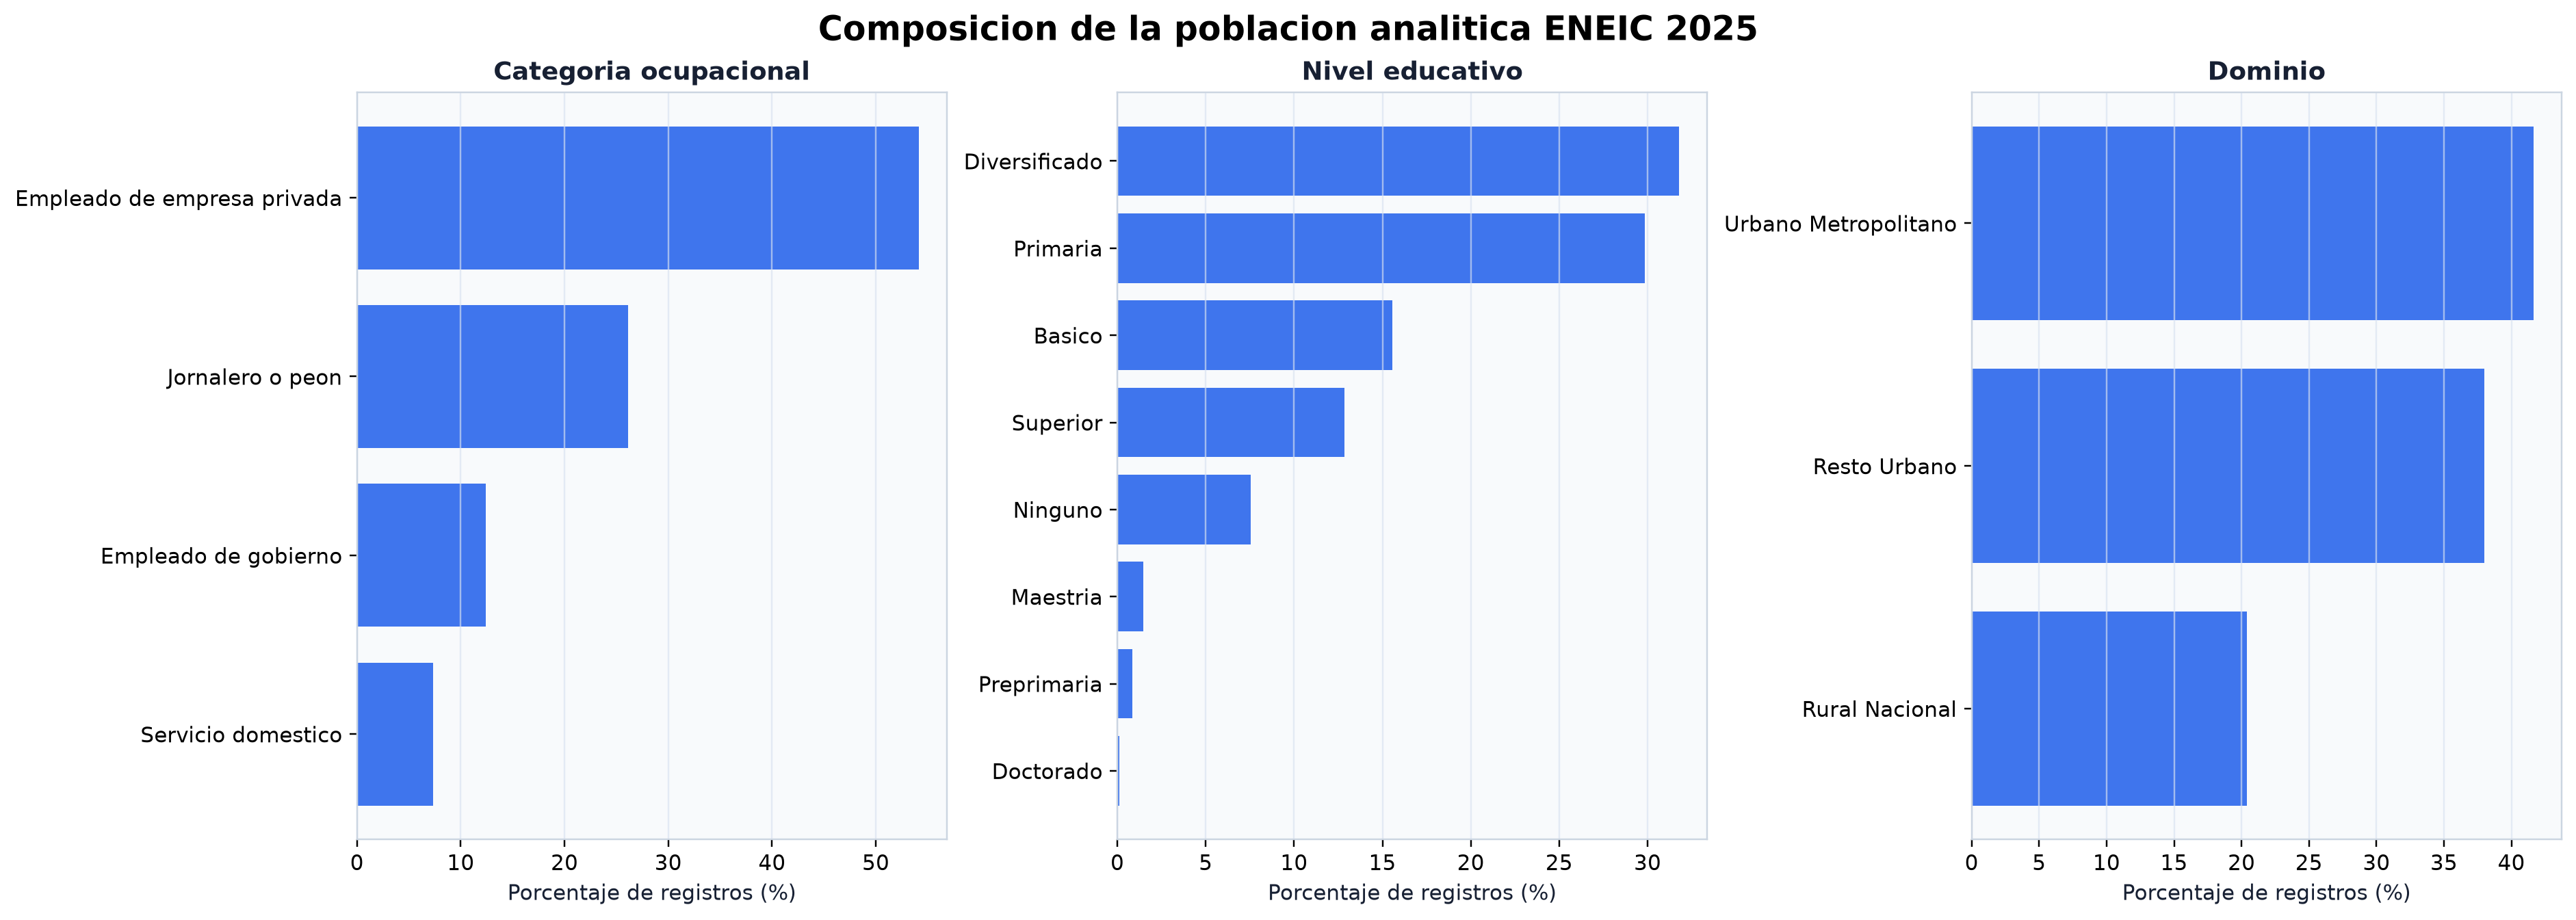
\includegraphics[width=\textwidth]{distribuciones_categoricas.png}
\caption{Composición de los registros elegibles de 2025.}
\end{figure}

\section{Exploración y relaciones}

\begin{figure}[htbp]
\centering
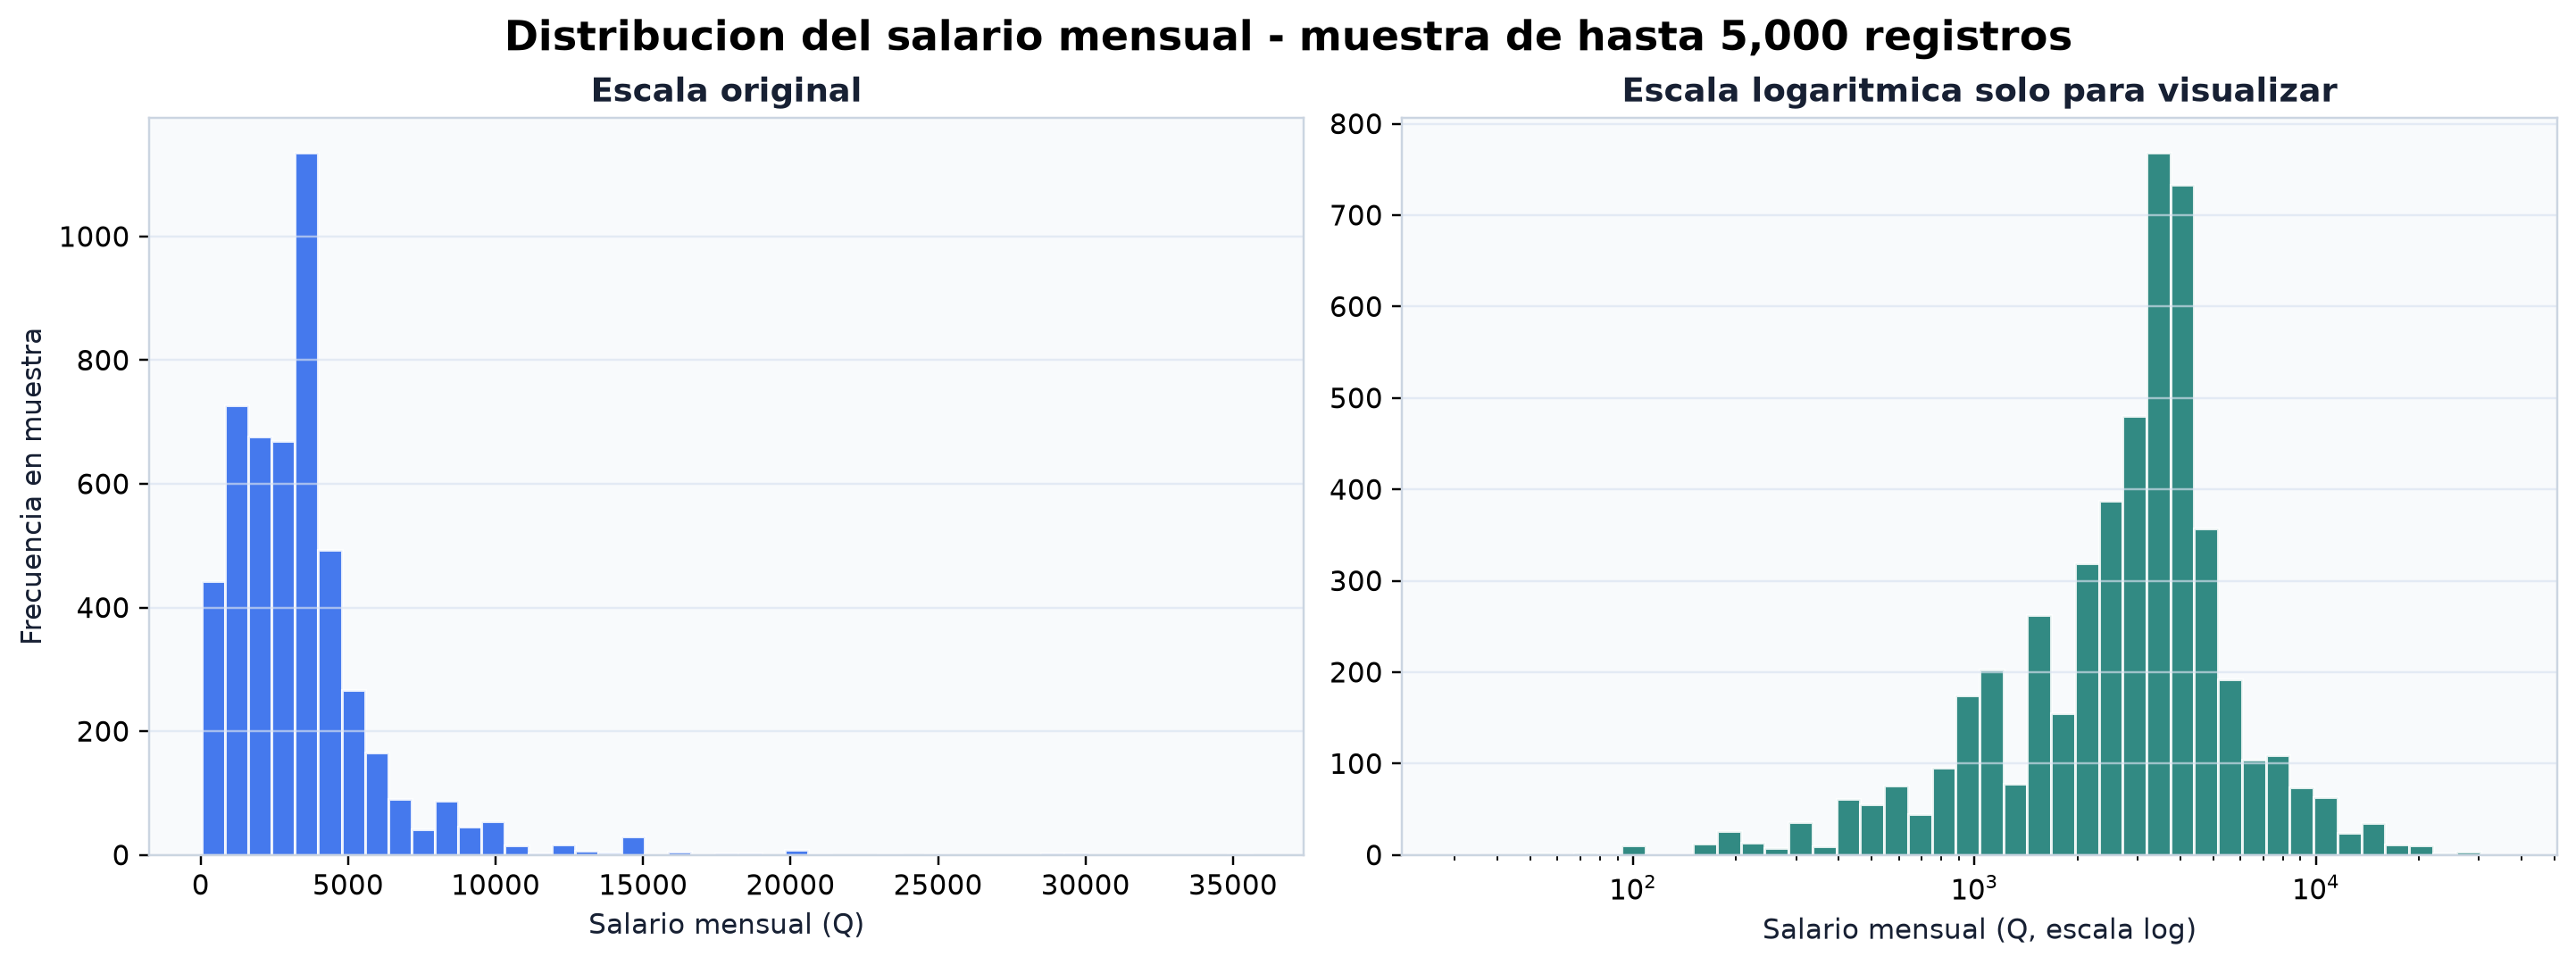
\includegraphics[width=\textwidth]{distribucion_salario.png}
\caption{Distribución salarial. La escala logarítmica se usa solo para visualización.}
\end{figure}

\begin{figure}[htbp]
\centering
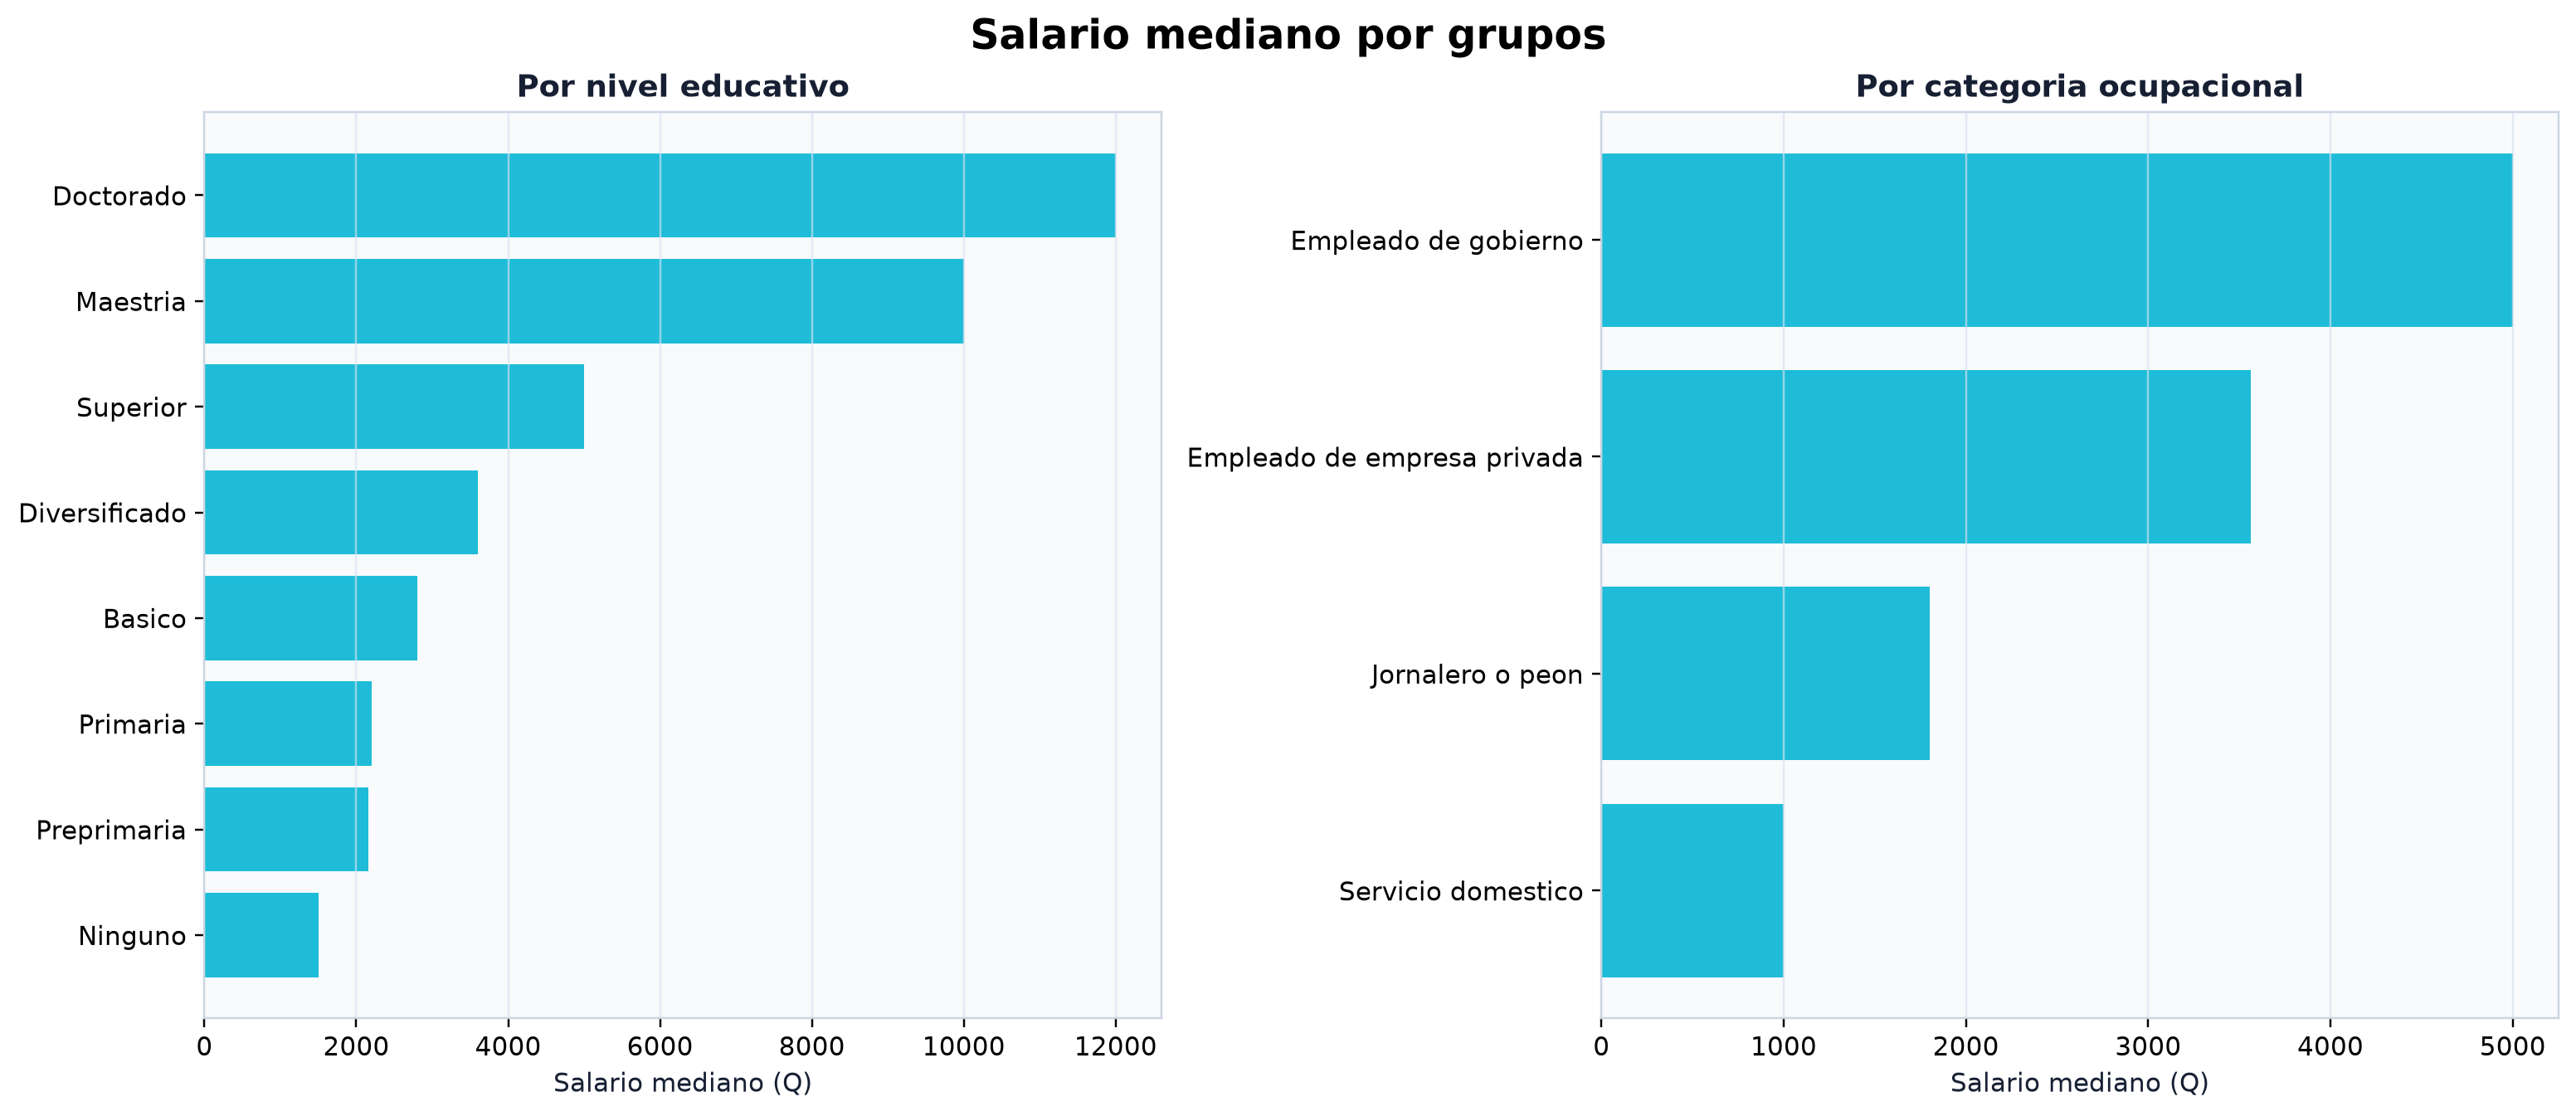
\includegraphics[width=0.92\textwidth]{salario_mediano_grupos.png}
\caption{Salario mediano por nivel educativo y categoría ocupacional.}
\end{figure}

\begin{figure}[htbp]
\centering
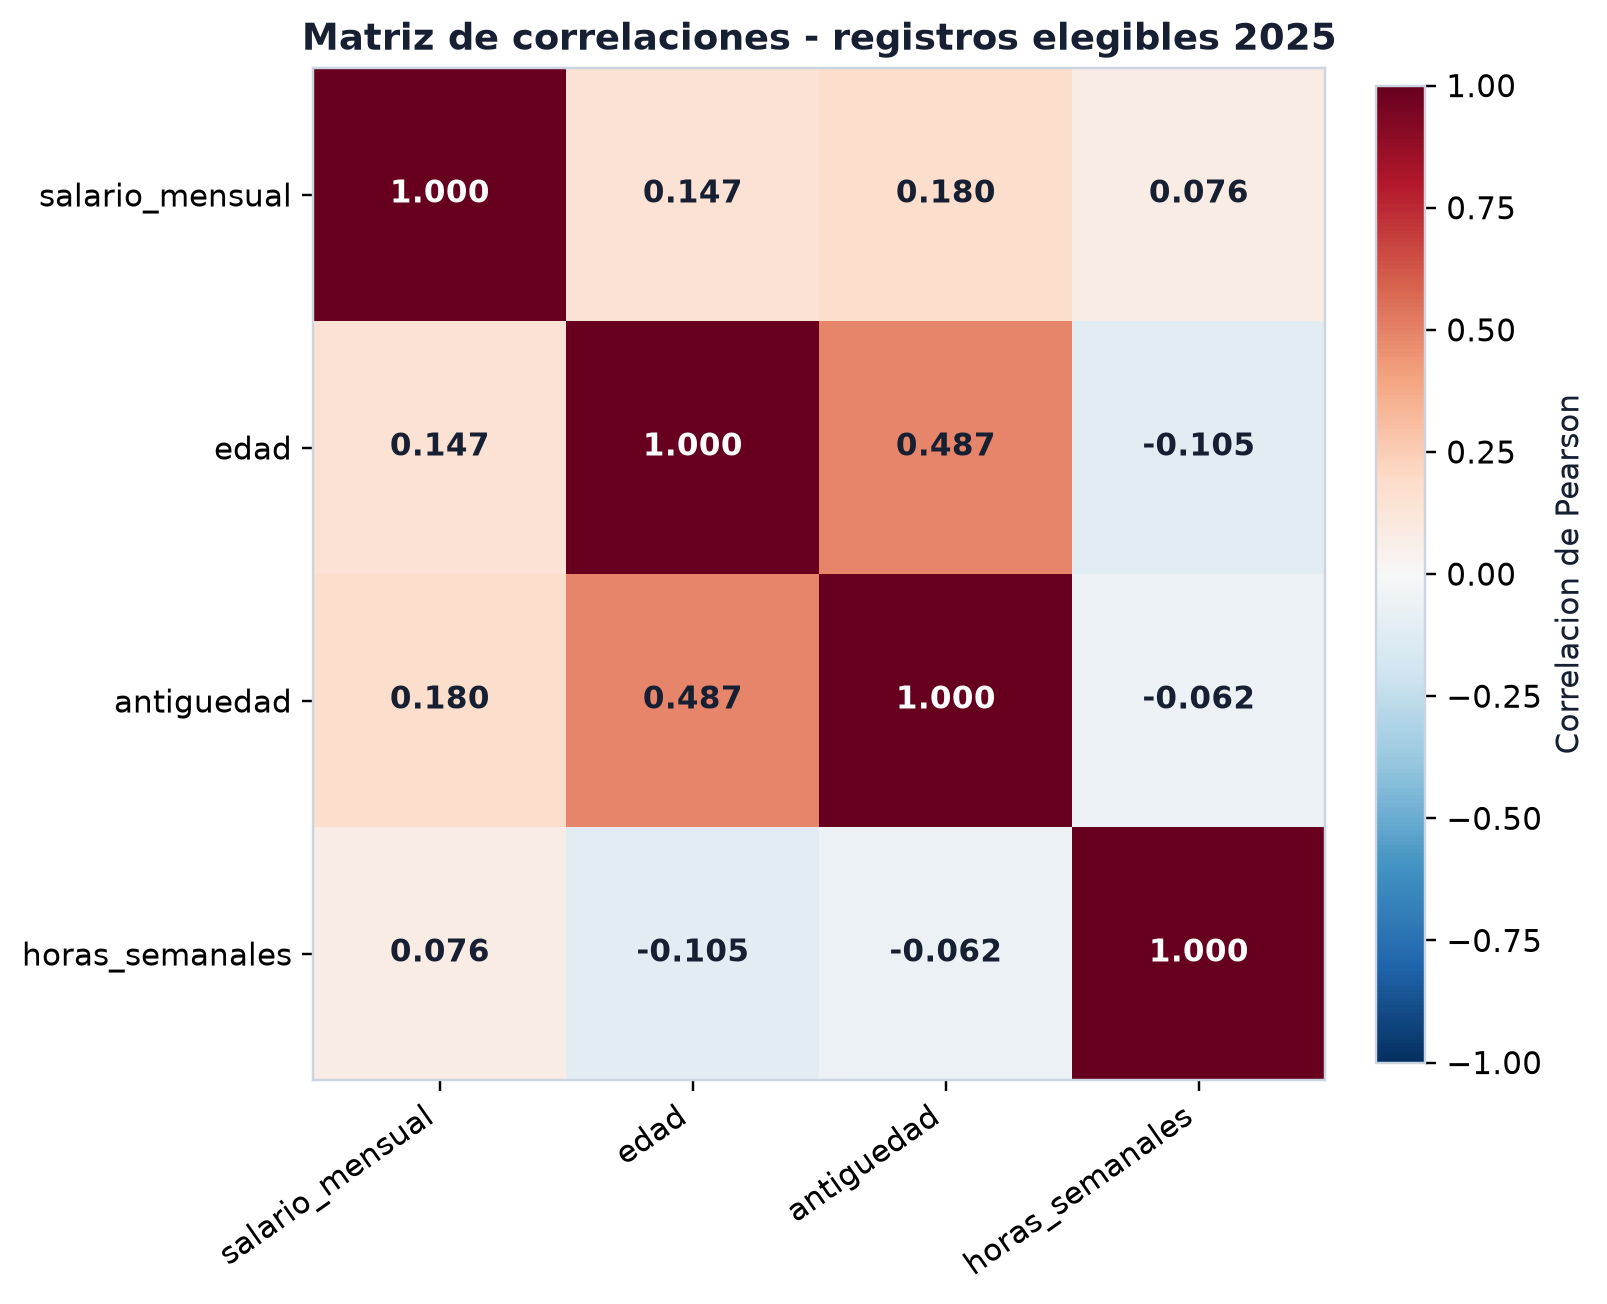
\includegraphics[width=0.78\textwidth]{correlaciones_pearson.png}
\caption{Correlaciones de Pearson calculadas con todos los registros elegibles de 2025.}
\end{figure}

\section{Segmentación KMeans}

Se estandarizaron las variables y se compararon $K=2,3,4,5$ tanto con un perfil laboral sin salario como con un perfil económico que lo incorpora. La elección se basa en silhouette; la descripción de los clústeres es relativa a las medias del conjunto y no representa categorías naturales.

\begin{figure}[htbp]
\centering
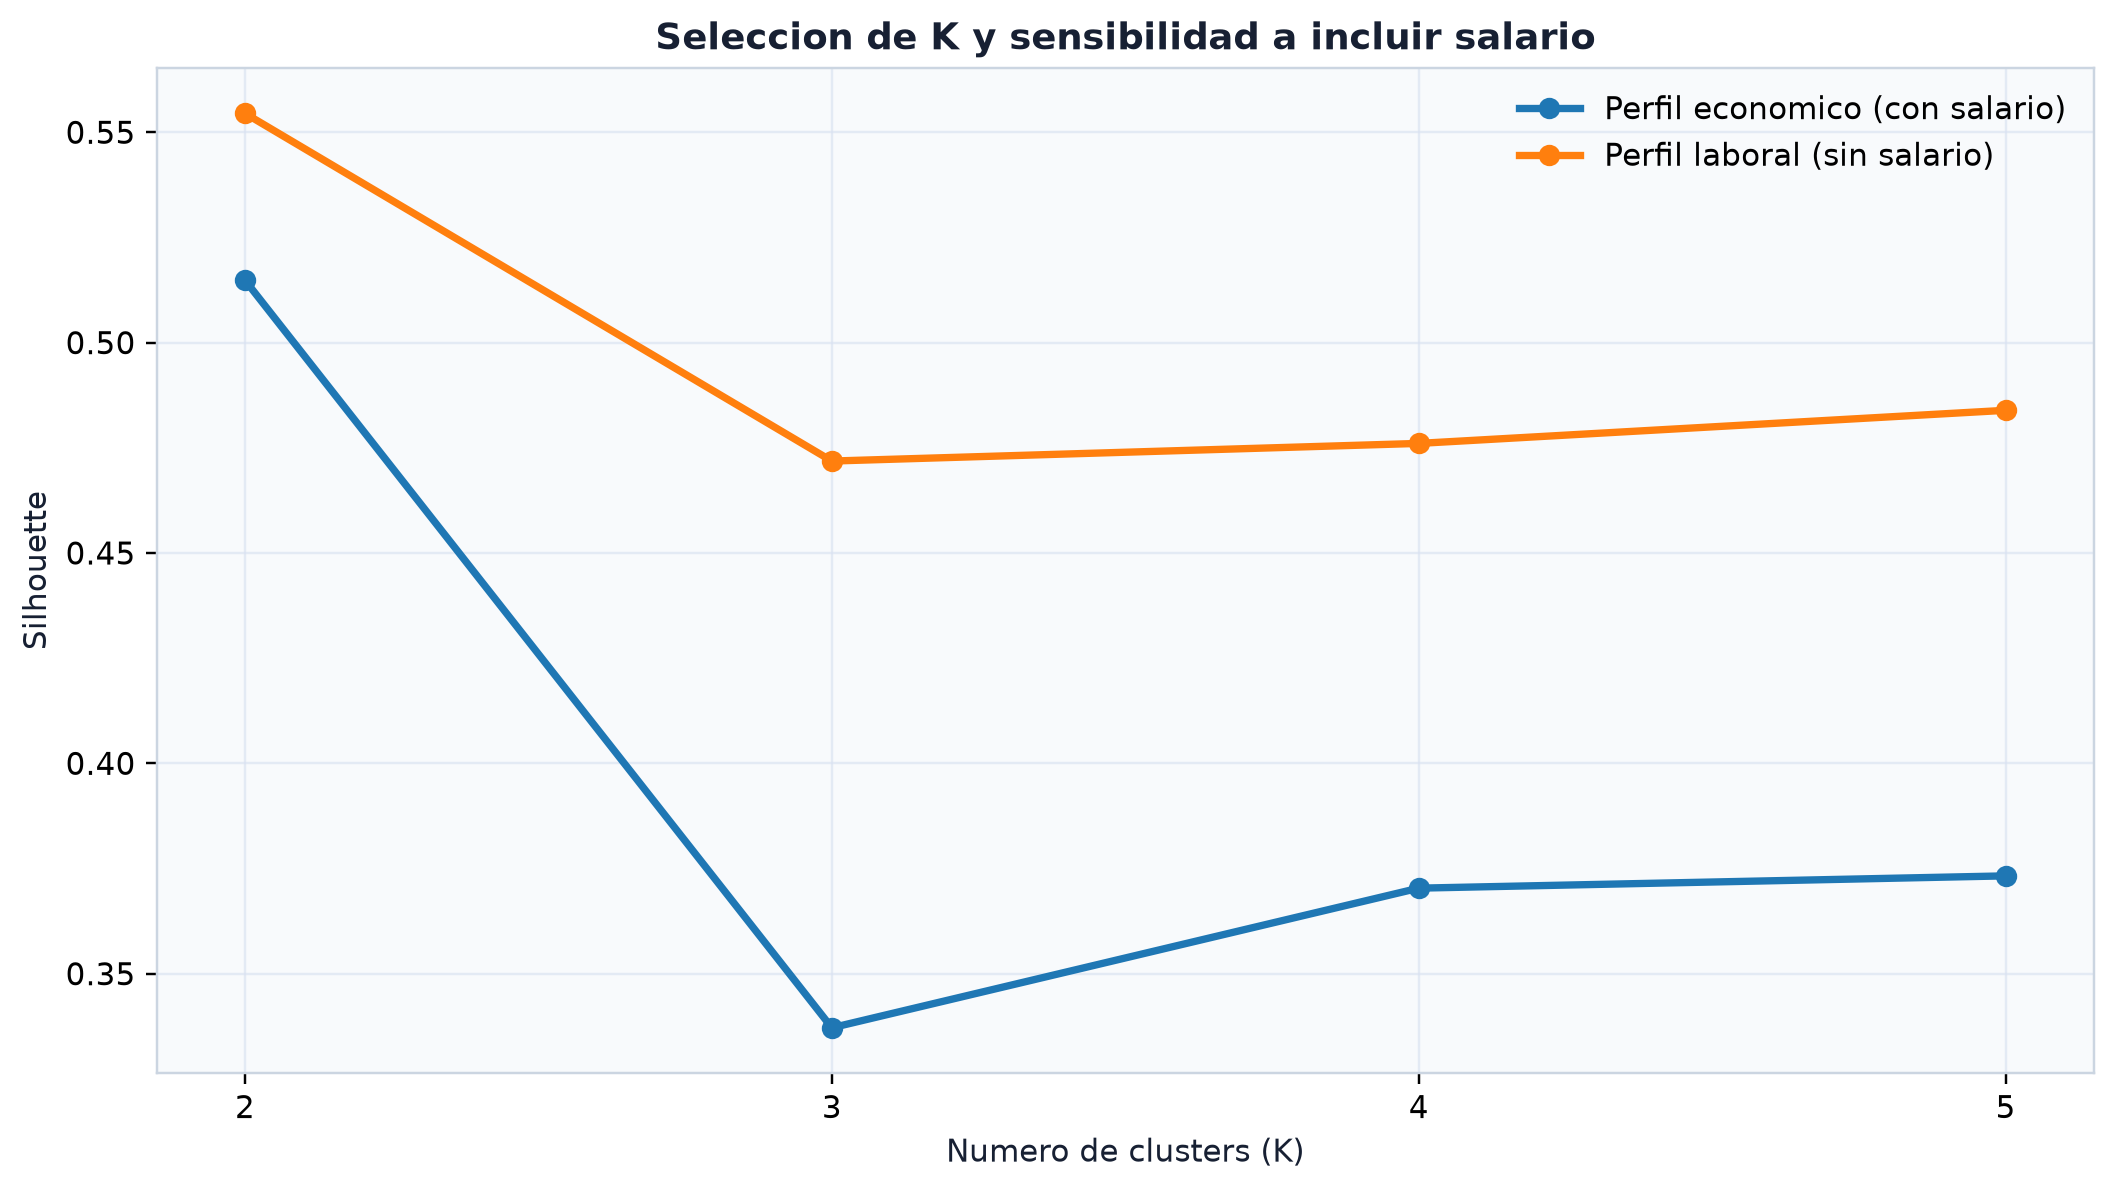
\includegraphics[width=0.82\textwidth]{seleccion_kmeans.png}
\caption{Selección de K y sensibilidad a la inclusión del salario.}
\end{figure}

\section{Modelado supervisado}

Los modelos utilizan exactamente edad, antigüedad, horas semanales, nivel educativo, categoría ocupacional y dominio. Se entrenó con 2025T1--T3 y se validó en 2025T4. Los indexadores, codificadores y estimadores se ajustaron solo con entrenamiento. La regresión lineal compara tres regularizaciones y Random Forest dos configuraciones de árboles y profundidad.

\begin{figure}[htbp]
\centering
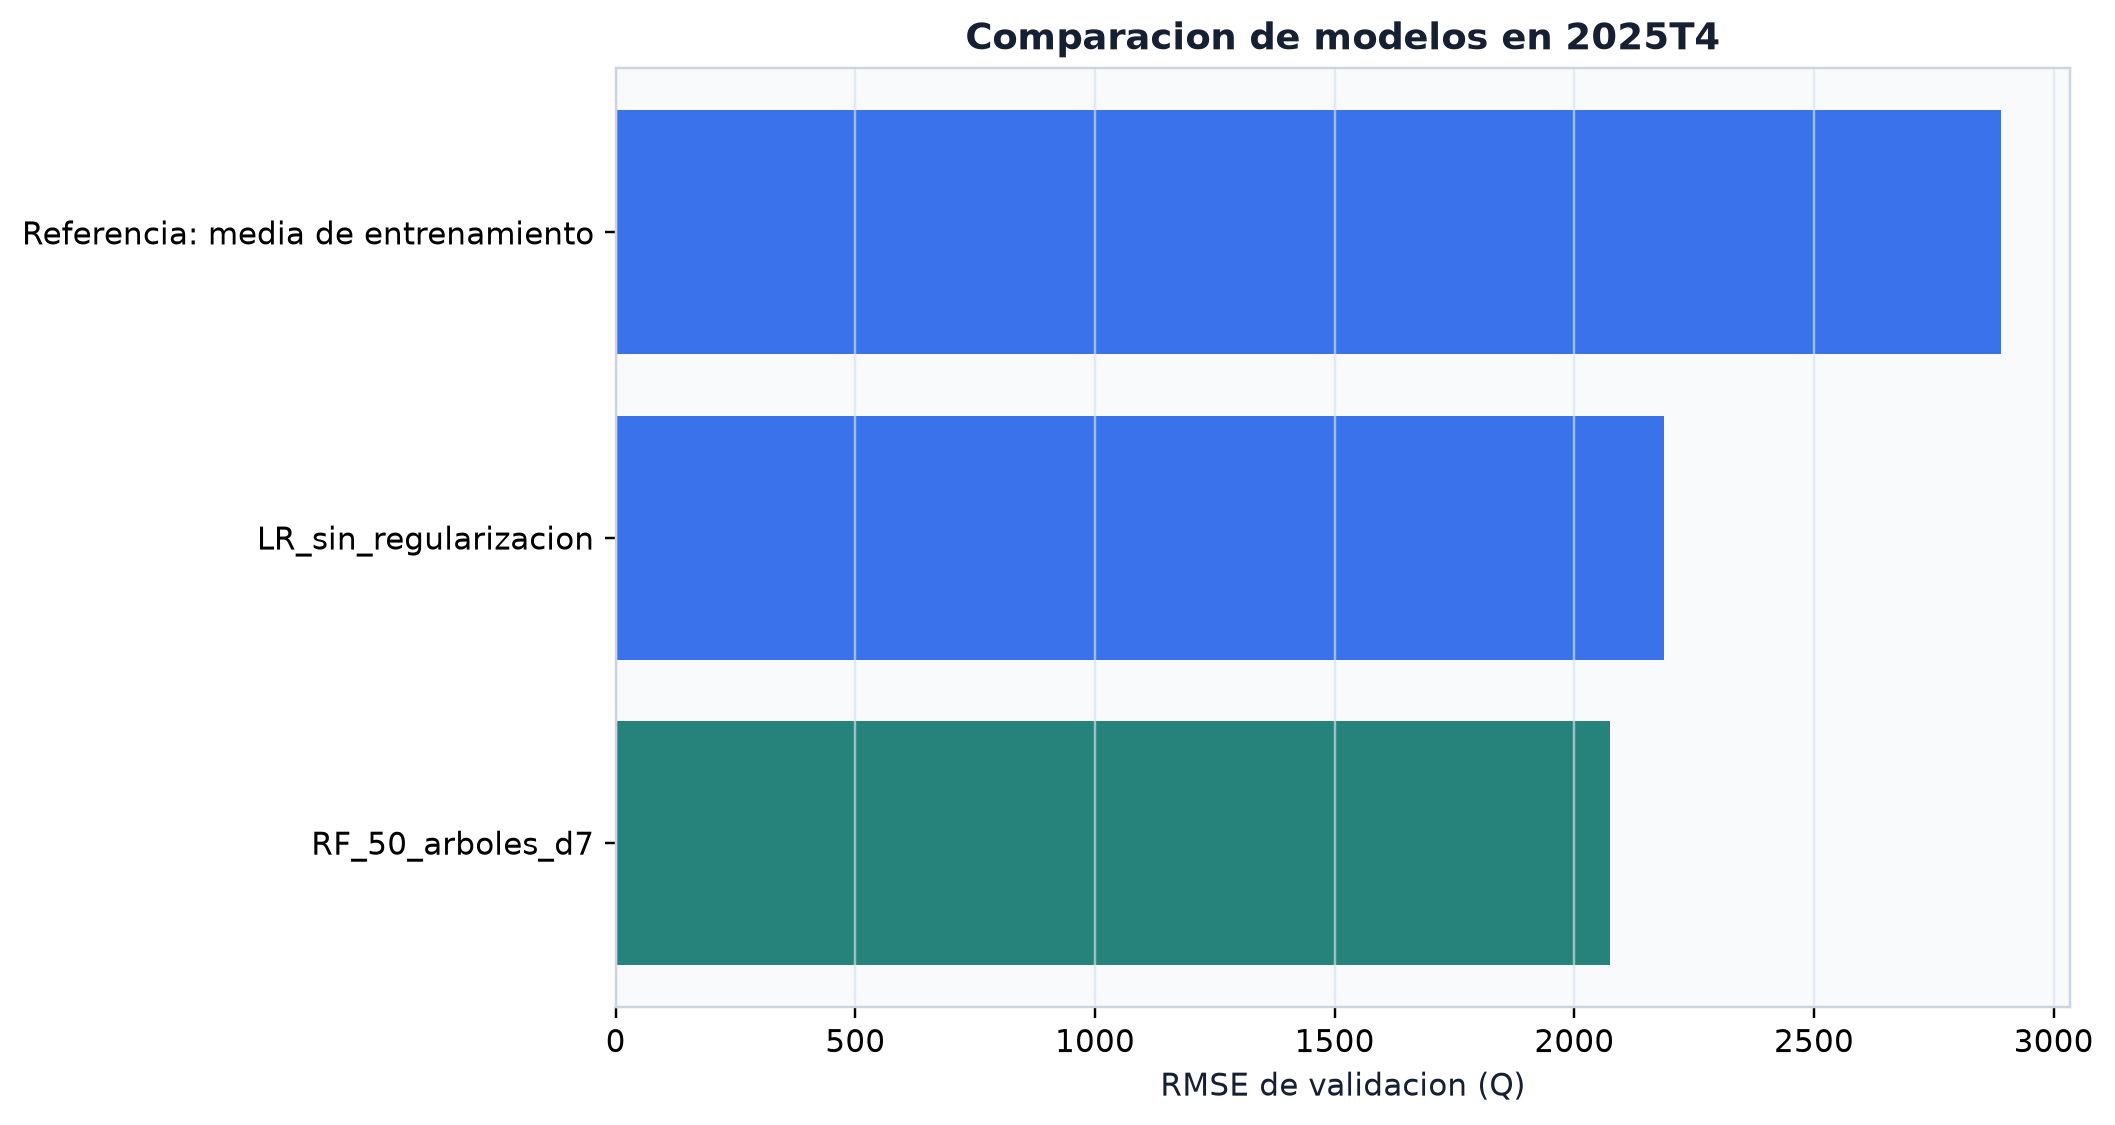
\includegraphics[width=0.86\textwidth]{comparacion_modelos_validacion.png}
\caption{RMSE de validación frente al modelo de referencia.}
\end{figure}

\section{Estado y trabajo restante}

Las actividades 1--6 están ejecutadas y sus modelos ganadores se guardaron fuera de Git. Para la entrega final se reentrenará cada configuración seleccionada con todo 2025, se evaluará una sola vez sobre 2026T1 y se completarán gráficos de predicción, residuos, errores por educación y dominio, análisis por percentiles y discusión final.

\section{Reproducibilidad y limitaciones}

El notebook fija semilla 42, mantiene el test temporal aislado y limita cualquier transferencia a pandas a agregados o una muestra gráfica de 5,000 filas. \texttt{FACTOR} se conserva para documentar el diseño, pero las métricas obligatorias son no ponderadas. El repositorio no incluye Excel, Parquet ni modelos por su tamaño; el README documenta las rutas y dependencias.

\section{Fuente}

Instituto Nacional de Estadística de Guatemala. \emph{Encuesta Nacional de Empleo e Ingresos Continua (ENEIC)}, bases de Personas 2025--2026.\\
\texttt{https://www.ine.gob.gt/encuesta-nacional-de-empleo-e-ingresos/}

Kassis, T., Agarwal, V., He, Y., Patel, D. y Brueckner, A. M. (2026). \emph{Scientific Agent Skills: A Library of Procedural Knowledge for Research Agents}. arXiv:2609.00065. DOI: \texttt{10.48550/arXiv.2609.00065}.

\end{document}
